% Layout adapted from the research memo shown in Lecture 1, sized for A4.
\documentclass[a4paper,10pt]{article}
\usepackage[margin=18mm,footskip=9mm]{geometry}
\usepackage{iftex}
\ifPDFTeX
  \usepackage[T1]{fontenc}
  \usepackage[utf8]{inputenc}
  \usepackage[scaled=0.96]{helvet}
  \renewcommand{\familydefault}{\sfdefault}
\else
  \usepackage{fontspec}
  \setmainfont{texgyreheros}[Extension=.otf,
    UprightFont=*-regular, BoldFont=*-bold,
    ItalicFont=*-italic, BoldItalicFont=*-bolditalic]
\fi
% For Chinese, set this switch true and compile with --engine xelatex.
\newif\ifChineseMemo
\ChineseMemofalse
\ifChineseMemo
  \ifPDFTeX
    \PackageError{finance-memo}{Chinese text requires XeLaTeX or LuaLaTeX}{}
  \else
    \usepackage[UTF8,fontset=fandol]{ctex}
    \renewcommand{\familydefault}{\sfdefault}
  \fi
\fi
\usepackage{booktabs,graphicx,xcolor,caption,xurl,fancyhdr}
\definecolor{MemoBlue}{HTML}{203E70}
\definecolor{MemoRule}{HTML}{B9C8DF}
\usepackage[colorlinks=true,linkcolor=MemoBlue,urlcolor=MemoBlue]{hyperref}
\captionsetup{font=small,labelfont=bf,skip=4pt}
\setlength{\parindent}{0pt}
\setlength{\parskip}{5pt}
\pagestyle{fancy}
\fancyhf{}
\renewcommand{\headrulewidth}{0pt}
\renewcommand{\footrulewidth}{0.3pt}

\newcommand{\ReportTitle}{NVDA FY2027 Q2: Underperform, target price \$186}
\newcommand{\ReportType}{EARNINGS UPDATE}
\newcommand{\ReportDate}{2026-11-14}
\newcommand{\DataDate}{2026-08-26 20:36:00 UTC}
\newcommand{\ReportScope}{Quarter ended 2026-07-26 (CY2026Q2); trigger filing 0001045810-26-000075}
\newcommand{\TeamName}{Semis Coverage (coursework)}
\newcommand{\DeskName}{AI semiconductor supply chain}
\newcommand{\ReportAuthor}{Coursework analyst (AI-assisted workflow)}
\newcommand{\Coverage}{NVDA, AMD, INTC, AVGO, MRVL, MU, AMAT}
\newcommand{\KeyFinding}{Revenue \$96.2bn (17.9\% q/q); target price \$186 vs last close \$209.66 (-11.3\%).}
\fancyfoot[L]{\scriptsize\TeamName}
\fancyfoot[R]{\scriptsize\ReportType}

\begin{document}
\begin{minipage}[t]{0.70\textwidth}
\vspace{0pt}
{\small\ReportDate}\par\medskip
{\color{MemoBlue}\hrule height 0.5pt}\smallskip
{\large\ReportType}\par
{\LARGE\bfseries\ReportTitle}\par\medskip
\ReportScope
\end{minipage}\hfill
\begin{minipage}[t]{0.23\textwidth}
\vspace{0pt}\raggedleft
\colorbox{MemoBlue}{\parbox[c][19mm][c]{0.86\linewidth}{\centering\color{white}\bfseries\TeamName}}\par\medskip
\DeskName
\end{minipage}
\par\bigskip
{\color{MemoBlue}\hrule height 0.5pt}\medskip
{\large\KeyFinding}\par\bigskip

\begin{minipage}[t]{0.61\textwidth}
\vspace{0pt}\raggedright
\setlength{\parskip}{4pt}
\textbf{Summary}\par
See key points and full note below. Figures are generated by code from SEC filings; prose is AI-drafted and human-approved.
\end{minipage}\hfill
\begin{minipage}[t]{0.36\textwidth}
\vspace{0pt}\small
% Author these non-floating wrappers separately. Use \captionof{table/figure},
% then a description and \input/\includegraphics of generated content.
\IfFileExists{sections/tables.tex}{\captionof{table}{Key data, FY2027 Q2}\label{tab:key-data}
{\footnotesize Reported figures for the quarter ended 2026-07-26 (CY2026Q2) from SEC XBRL facts; NTM, DCF and target price are model outputs. US\$.\par}
\begin{tabular}{@{}lr@{}}
\toprule
Item & Value \\
\midrule
Revenue (quarter) & \$96.2bn \\
Revenue q/q & 17.9\% \\
Revenue y/y & 105.9\% \\
Gross margin & 75.0\% \\
Operating margin & 66.2\% \\
Diluted EPS & \$2.46 \\
Free cash flow & \$21.4bn \\
\midrule
NTM revenue (model) & \$492.4bn \\
NTM EPS (model) & \$11.10 \\
DCF value / share & \$141.68 \\
Peer EV/Sales (median) & 23.0x \\
Last close & \$209.66 \\
Target price & \$186 \\
Upside & -11.3\% \\
Rating & Underperform \\
\bottomrule
\end{tabular}

}{
  \textbf{Key data}\par
  [Insert a compact checked table, including units and periods.]
}
\medskip
\IfFileExists{sections/figures.tex}{\captionof{figure}{Quarterly revenue, reported and forecast}\label{fig:revenue}
{\footnotesize Solid: reported (SEC XBRL, fiscal quarters). Hatched: model forecast from this case's assumptions. US\$ bn.\par}
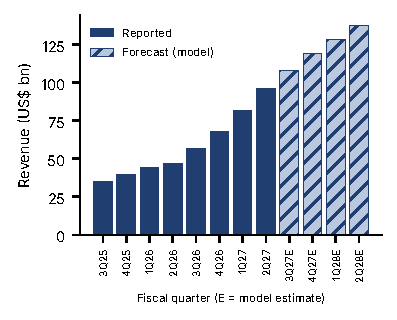
\includegraphics[width=\linewidth]{../../output/figures/NVDA-0001045810-26-000075-r2/revenue.pdf}
}{
  \textbf{Supporting chart}\par
  [Insert a chart with readable labels, units, and a source note.]
}
\end{minipage}
\par\bigskip

Fiscal quarter FY2027 Q2 / calendar quarter CY2026Q2, quarter ended 2026-07-26. In this note, "reported" means figures from SEC XBRL facts or derived from them by code, "forecast" means our model outputs, and "judgment" marks analyst opinion.

\par\smallskip\textbf{\color{MemoBlue}Key points}\par

\begin{itemize}\setlength{\itemsep}{1pt}
\item \textbf{Reported:} revenue was \$96.2bn, up 17.9\% sequentially and 105.9\% year on year. Gross margin was 75.0\%, operating margin 66.2\% and diluted EPS \$2.46. Data Center remained the driver: “Data Center revenue for the second quarter was a record \$89.0 billion, up 117\% from a year ago and up 18\% sequentially, driven by the ramp of our Blackwell Ultra infrastructure.”
\item \textbf{Company guidance:} for FY2027Q3 the company guides revenue of \$108.0bn and gross margin of 74.0\% (midpoints). The outlook excludes China: “We are not assuming any Data Center compute revenue from China in our outlook.”
\item \textbf{Forecast:} our model gives next-twelve-month revenue of \$492.4bn and NTM EPS of \$11.10. Only FY2027Q3 is anchored on guidance. The three quarters after it are our judgments, not company guidance.
\item \textbf{Valuation (code output):} the blended target price of \$186 is -11.3\% against the last close of \$209.66. Under the rating bands in the Disclosures, that maps mechanically to Underperform. \textbf{Judgment:} the rating reflects valuation, not a negative view of the quarter's quality. The upside sits close to the Underperform/Neutral boundary.
\end{itemize}

\par\smallskip\textbf{\color{MemoBlue}Results}\par

\textbf{Reported.} Revenue for FY2027 Q2 was \$96.2bn (17.9\% q/q, 105.9\% y/y), bringing trailing-twelve-month revenue to \$303.0bn. Gross margin was 75.0\%. Management described margins this way: “GAAP and non-GAAP gross margins were approximately flat sequentially as our Blackwell architecture remains the vast majority of our revenue.” Operating margin was 66.2\%, net income \$59.7bn and diluted EPS \$2.46. Free cash flow (operating cash flow less capital expenditure) was \$21.4bn for the quarter.

\textbf{Balance sheet and working capital (reported, from the CFO commentary).} “Inventory was \$31.6 billion, up from \$25.8 billion sequentially, as we prepare for the introduction of Vera Rubin in the third quarter.” “Accounts receivable was \$63.1 billion with 60 days sales outstanding (DSO), up from 45 days sequentially, due to extended payment terms on large, multi-quarter agreements with certain investment-grade customers.” Capital return continued: “During the second quarter of fiscal 2027, NVIDIA returned approximately \$26.0 billion to shareholders in the form of shares repurchased and cash dividends.”

\textbf{Net cash (code output).} Net cash is \$66.0bn. It is cash and cash equivalents plus current marketable securities, less total debt (the debt figure includes both the short-term and long-term portions). Current marketable securities now include both marketable debt securities and marketable equity securities. \textbf{Judgment:} the marketable equity securities are carried at fair value, so they move with market prices, and their realisable value at any later date may differ materially from the balance-sheet figure. Non-current non-marketable investments and operating lease liabilities are left out of net cash. On the asset side that is conservative.

\par\smallskip\textbf{\color{MemoBlue}Guidance and outlook}\par

\textbf{Company guidance for FY2027Q3 (quoted):}

\begin{itemize}\setlength{\itemsep}{1pt}
\item Revenue: “Revenue is expected to be \$108.0 billion, plus or minus 2\%.”
\item Gross margin: “GAAP and non-GAAP gross margins are expected to be 74.0\%, plus or minus 50 basis points.”
\item Operating expenses: “GAAP and non-GAAP operating expenses are expected to be approximately \$9.2 billion and \$9.0 billion, respectively.”
\item Tax rate: “For the full year fiscal 2027, we expect GAAP and non-GAAP tax rates to be between 16.0\% and 18.0\%, excluding any discrete items and material changes to our tax environment.”
\item China: “We are not assuming any Data Center compute revenue from China in our outlook.”
\end{itemize}

\textbf{Our forecast.} FY2027Q3 revenue is \$108.0bn, which is the guidance midpoint (\$108.0bn). Gross margin is the 74.0\% midpoint, and the full-year tax rate is the 17.0\% midpoint of the guided range. Operating expenses follow the GAAP guide of \$9.2bn (non-GAAP \$9.0bn). That gives forecast FY2027Q3 EPS of \$2.42.

\textbf{Judgment.} We have no company guidance for the quarters after FY2027Q3. For those quarters we extend the recent deceleration in sequential revenue growth, hold gross margin at the guided level and let operating expenses grow more slowly than revenue. These are analyst judgments, not guidance. Like the company's outlook, our forecast assumes no China Data Center compute revenue in any quarter. Any resumption of those sales would be upside to the model; none is assumed. The guided step-down in gross margin from the 75.0\% reported coincides with the Vera Rubin introduction. We assume neither further dilution nor a recovery.

\par\smallskip\textbf{\color{MemoBlue}Model and valuation}\par

\textbf{Forecast.} NTM revenue is \$492.4bn and NTM EPS is \$11.10. The model applies the guided tax rate to operating income and assumes no other income or expense. It ignores interest income and gains or losses on investments, including the fair-value changes on marketable equity securities.

\textbf{Valuation (code output).} The target price of \$186 blends two methods, with the larger weight on the DCF:

\begin{itemize}\setlength{\itemsep}{1pt}
\item A DCF value of \$141.68 per share. The terminal value makes up 71\% of DCF enterprise value.
\item A peer cross-check that applies the peer median TTM EV/Sales of 23.0x (AMD, Broadcom, Marvell) to NVIDIA's TTM revenue of \$303.0bn.
\end{itemize}

Net cash of \$66.0bn is added to enterprise value. Against the last close of \$209.66, the implied upside is -11.3\%, which gives a rating of Underperform.

\textbf{Judgment.} The discount rate, the long-run FCF margins and the terminal growth rate are analyst assumptions. Market-rate inputs are not in the case snapshot, so the discount rate is built from assumed risk-free, beta and equity-risk-premium inputs. Terminal value carries most of the DCF, and the upside is close to the band boundary. A modestly lower discount rate would therefore move the result from Underperform into Neutral. We do not regard the rating as a high-conviction call. The peer multiple sets NVIDIA's revenue against companies with lower margins. The peers' latest reported trailing-twelve-month periods also end one to three months before NVIDIA's quarter end. For both reasons the peer cross-check gets the smaller weight.

\par\smallskip\textbf{\color{MemoBlue}Risks}\par

\begin{itemize}\setlength{\itemsep}{1pt}
\item \textbf{Commitments and guarantees (reported):} “Our commitments increased from \$119 billion last quarter to \$279 billion, primarily related to the procurement of memory.” “Our guarantee obligations are capped at a total of \$105 billion and become effective in phases as certain conditions are met, including data centers becoming ready for service, with the first expected in fiscal 2029.” \textbf{Judgment:} these magnify the effect of any slowdown in AI infrastructure spending on cash flow and margins.
\item \textbf{Customer concentration and credit terms:} “Accounts receivable was \$63.1 billion with 60 days sales outstanding (DSO), up from 45 days sequentially, due to extended payment terms on large, multi-quarter agreements with certain investment-grade customers.” \textbf{Judgment:} the longer payment terms on large multi-quarter agreements tie up working capital and point to dependence on a small set of very large customers.
\item \textbf{China and export controls:} the outlook assumes no China Data Center compute revenue (“We are not assuming any Data Center compute revenue from China in our outlook.”). Further restrictions or changes to them remain a two-way risk.
\item \textbf{Product transition:} the Vera Rubin ramp (“Inventory was \$31.6 billion, up from \$25.8 billion sequentially, as we prepare for the introduction of Vera Rubin in the third quarter.”) brings execution and margin risk. This is already visible in the guided gross-margin step-down to 74.0\%.
\item \textbf{Valuation and model risk (judgment):} terminal value is 71\% of DCF enterprise value, and the rating sits near a band boundary. Net cash includes marketable equity securities at fair value, and their value moves with market prices.
\item \textbf{Upside risks (judgment):} our growth after FY2027Q3 could prove too conservative. China data-center sales could resume. Gross margin could recover after the transition.
\end{itemize}

\par\smallskip\textbf{\color{MemoBlue}Disclosures}\par

\begin{itemize}\setlength{\itemsep}{1pt}
\item For coursework demonstration only; not investment advice.
\item Data sources and as-of times. The case was triggered by NVIDIA's SEC EDGAR 10-Q for the quarter ended 2026-07-26. Its accession number and the exact SEC acceptance timestamp are recorded in the case manifest and printed in the published report's data-source line. The note's provenance gate admits no digits other than code values, so they are not repeated here. The information cutoff is the SEC acceptance time of that 10-Q on August twenty-sixth, 2026 (UTC), and no information after it is used. The guidance and commentary quotes come from the earnings-release exhibits (EX-99.1, EX-99.2) of a separate company 8-K, which was accepted before the cutoff. The share price of \$209.66 is the close of the August twenty-sixth, 2026 session, the last close whose session ended before the cutoff (Yahoo chart endpoint, case price snapshot).
\item Rating definitions: Outperform means upside to the target price of fifteen percent or more. Underperform means upside of minus ten percent or lower. Neutral covers everything in between.
\item All figures in this note are generated by code from SEC XBRL data (and, for guidance, taken from verbatim filing quotes) and are unaudited by the author. Forecasts and valuation depend on the analyst assumptions and judgments set out above.
\end{itemize}
\par\vfill

{\color{MemoRule}\hrule height 0.4pt}\medskip
\begin{minipage}[t]{0.36\textwidth}
\vspace{0pt}\small
\setlength{\parskip}{3pt}
\textbf{PREPARED BY}\par\ReportAuthor\par\TeamName\par
\medskip\textbf{COVERAGE}\par\Coverage
\end{minipage}\hfill
\begin{minipage}[t]{0.60\textwidth}
\vspace{0pt}\footnotesize
\setlength{\parskip}{3pt}
\textbf{Sources and dates.} Data as of \DataDate.
SEC EDGAR filings accepted at or before 2026-08-26T20:36:00Z (trigger 0001045810-26-000075); last close \$209.66 on the cutoff date from the Yahoo chart endpoint. Case files: cases/NVDA-0001045810-26-000075-r2.

\textbf{Checks.} Numerical and provenance gates passed; two consecutive clean reviews by three independent critics (round 1); approved by Repository owner (kuostudy31-bot); executed by Claude under the owner's delegation of 2026-11-14 on 2026-11-14.

\textbf{Preparation.} Claude Code agent team (orchestrator, generator and critic leads, eight specialists) under a Python controller; for coursework demonstration only, not investment advice.
\end{minipage}
\end{document}
